\documentclass{article}
\usepackage[submission]{colm2026_conference}
\usepackage{microtype}
\usepackage{hyperref}
\usepackage{url}
\usepackage{booktabs}
\usepackage{lineno}
\usepackage{graphicx}
\usepackage{wrapfig}
\usepackage{amsmath}
\usepackage{subcaption}
\usepackage{xcolor}
\definecolor{darkblue}{rgb}{0,0,0.5}
\hypersetup{colorlinks=true, citecolor=darkblue, linkcolor=darkblue, urlcolor=darkblue}

% tighten space around floats and captions to respect the 4-page main-body limit
\setlength{\textfloatsep}{5pt plus 2pt minus 2pt}
\setlength{\intextsep}{5pt plus 2pt minus 2pt}
\setlength{\abovecaptionskip}{3pt}
\setlength{\belowcaptionskip}{0pt}

\title{Low-Cost Geometric Directions in Frozen Speech Models:
Where a Training-Free Deepfake-Hardness Signal Helps---and Where It Does Not}

\author{Anonymous authors\\Paper under double-blind review}

\begin{document}
\linenumbers
\maketitle

\begin{abstract}
Deepfake-speech detectors are inconsistent in two systematic ways: against a fixed
detector some synthesis systems evade detection far more often than others, and a
detector trained on one recording domain often fails on another. Working entirely
at small scale---one GPU, a frozen $\sim$95M-parameter encoder, no detector
retraining---we show that much of this inconsistency is legible in the
\emph{geometry} of the frozen representation. Inside the encoder there is a single
natural-versus-synthetic direction, and how far a synthesis system's utterances
\emph{spread} along it predicts how hard that system is to detect---the only
quantity, out of 83 we tested, to survive a global false-discovery-rate correction.
Two further results follow. The direction is not universal: it rotates across
datasets to near-orthogonality, the geometric reason detectors fail to transfer.
And it is a training-free corrective signal conditional on headroom: it cuts a weak
detector's error by $\approx$21\% while leaving an already-strong one unchanged.
Every quantitative claim is independently recomputed.
\end{abstract}

\section{Introduction}
Synthetic speech is now realistic enough that its detection is a security
necessity, and the standard defence is a classifier that flags synthetic
utterances. Yet detectors are unreliable in two ways that aggregate accuracy hides:
some synthesis systems evade a fixed detector far more often than others
\citep{wang2020asvspoof,muller2024harder}, and a detector tuned on one recording
domain often fails on another \citep{muller2022wild}. Neither had a clean
explanation.

We provide one, at small scale. Modern detectors sit on top of a large frozen
self-supervised (SSL) speech encoder
\citep{chen2022wavlm,tak2022automatic,wang2022sslfrontend}; we study that frozen
representation before any decision boundary is drawn. Our central finding is a
\textbf{natural-versus-synthetic axis}, a single direction from natural to
synthetic speech: a system whose utterances stay tight along it is detected
easily, one whose utterances spread along it is hard (Fig.~\ref{fig:concept}).
That spread, $\mathrm{sd}_{\mathrm{along}}$, is our predictor. Three results
follow. (i)~\emph{The law:} $\mathrm{sd}_{\mathrm{along}}$ predicts per-system
hardness and is the only one of 83 tested quantities to survive global
multiple-testing correction (Sec.~\ref{sec:results}). (ii)~\emph{The axis
rotates:} each dataset has its own axis, so a transferred axis is
uninformative---the geometric reason transfer fails. (iii)~\emph{A training-free
corrective signal:} fusing the axis into a detector's score needs no detector
training and no difficulty labels, and helps only when the detector has headroom
(Sec.~\ref{sec:lever}). Every reported number was independently recomputed from
cached artifacts (Sec.~\ref{sec:audit}).

\section{Setup}
\label{sec:setup}

\begin{wrapfigure}{r}{0.35\linewidth}
\centering
\vspace{-12pt}
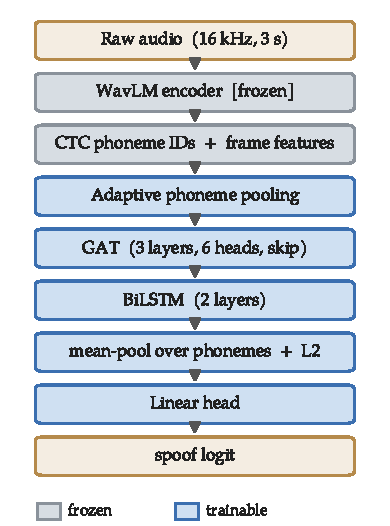
\includegraphics[width=\linewidth]{figs/fig1_architecture.pdf}
\vspace{-16pt}
\caption{The WavLM-GAT detector, redrawn after \citet{zhang2025phoneme}. A frozen
encoder feeds a small trainable head. All geometry is read from the frozen
layer-12 space.}
\label{fig:arch}
\vspace{-14pt}
\end{wrapfigure}

\textbf{Detector.} Our primary detector (WavLM-GAT) is the phoneme-level
graph-attention model of \citet{zhang2025phoneme}: a frozen WavLM encoder feeds
adaptive phoneme pooling, a 3-layer 6-head graph-attention network
\citep{velickovic2018graph}, a BiLSTM, and a linear head (Fig.~\ref{fig:arch}).
The encoder is frozen ($\sim$95M parameters; WavLM-base, 94.7M); only the
$\sim$13M-parameter head trains. For architecture generality we also use AASIST
\citep{jung2022aasist}, a spectro-temporal detector \emph{not} built on WavLM.

\textbf{Corpora and hardness.} The law is established on MLAAD
\citep{muller2024mlaad} (61 text-to-speech systems, $\geq 8$ utterances each); the
lever and rotation check add ASVspoof~2019~LA \citep{wang2020asvspoof}. Per-system
hardness is $1-\mathrm{AUC}$ of the detector's scores for that system against a
shared bona-fide pool. Class overlap is exactly what lowers AUC, so a geometric
``spread across the boundary'' should map onto hardness.

\textbf{Objective hardness.} Per-system hardness is a stable target, not a quirk of
one run. Three independently seeded WavLM-GAT detectors on MLAAD agree on the
per-system hardness ranking at Spearman $\rho=0.89$--$0.97$ (pairwise, 61 systems);
on ASVspoof~2019~LA the three seeds converge on essentially the same ranking
($\rho=0.94$--$1.00$, zero difficulty-category flips). Hardness is a property of the
(architecture, recording domain) pair, worth predicting, not of a random seed.

\textbf{Compute.} Everything runs on one GPU; the largest single training run is
$\approx 10^{16}$ FLOPs (well under the $10^{20}$ budget and $3$B-parameter cap).

\section{Experiments}
\label{sec:exp}

\subsection{The axis and its spread}
\label{sec:axissetup}

\begin{wrapfigure}{r}{0.35\linewidth}
\centering
\vspace{-14pt}
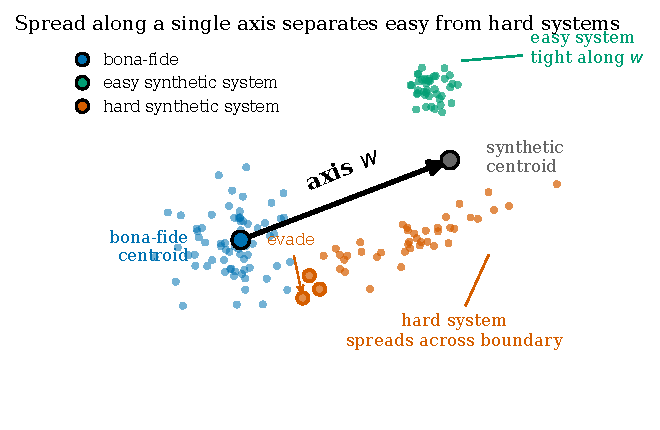
\includegraphics[width=\linewidth]{figs/fig1_concept.pdf}
\vspace{-16pt}
\caption{An easy system stays tight along $w$; a hard system spreads across the
boundary, so some utterances land in the bona-fide region and evade. Spread, not
mean position, is the predictor.}
\label{fig:concept}
\vspace{-12pt}
\end{wrapfigure}

\textbf{Frozen embeddings.} For each utterance (16~kHz, 3\,s) we take the frozen
WavLM layer-12 hidden states and mean-pool over time, one 768-dimensional vector
per clip. We read geometry from layer~12 because information in SSL encoders
stratifies from acoustic detail in early layers to linguistic content in deep
layers \citep{pasad2021layerwise,pasad2024words}: the natural-versus-synthetic
distinction is linguistic, so the deepest layer is where it should---and
empirically does---live. Each coordinate is standardized by the training
bona-fide mean and standard deviation, so none dominates through raw scale.

\textbf{The axis.} Per corpus we estimate the direction as the standardized
centroid difference
$w=\mathrm{centroid}(\text{synthetic})-\mathrm{centroid}(\text{bona})$---a
two-group mean difference, not a trained classifier: it uses the bona/synthetic
\emph{group} labels but no fitted decision boundary and no per-system difficulty
labels. We estimate $w$ corpus-internally (the direction differs across corpora,
Sec.~\ref{sec:results}) and \textbf{leave-one-system-out} (LOSO): when scoring a
system we rebuild $w$ from the bona pool plus every \emph{other} system's
synthetic clips, so a held-out system never informs the axis used to judge it---
without LOSO a system would help define the ruler it is graded on. For each system
we record $\mathrm{sd}_{\mathrm{along}}$, the standard deviation of its projections
onto $w$; the mechanism (Fig.~\ref{fig:concept}) predicts this second moment beats
mean position.

\subsection{Results: the law and its rotation}
\label{sec:results}

\begin{figure}[t]
\centering
\begin{subfigure}[t]{0.42\linewidth}
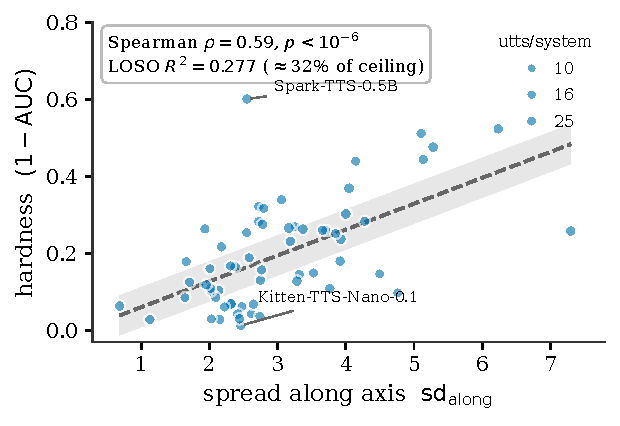
\includegraphics[width=\linewidth]{figs/fig2a_law_scatter.pdf}
\caption{The hardness law (MLAAD, 61 systems).}
\label{fig:law}
\end{subfigure}\hfill
\begin{subfigure}[t]{0.35\linewidth}
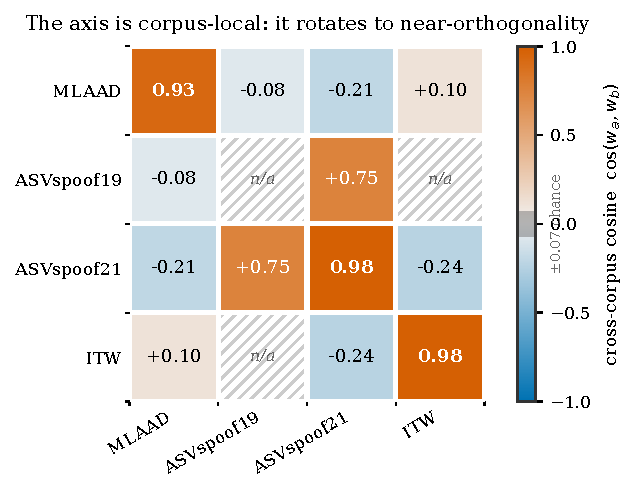
\includegraphics[width=\linewidth]{figs/fig2b_axis_rotation.pdf}
\caption{The axis is corpus-local.}
\label{fig:rotate}
\end{subfigure}
\caption{\textbf{(a)}~Spread along the corpus-internal axis predicts MLAAD
hardness. \textbf{(b)}~Cosine between per-corpus axes: within-corpus split-half
reliability on the diagonal ($0.93$--$0.98$); cross-corpus cosines near zero or
negative, inside/at the $\pm0.07$ chance band---a transferred axis is
uninformative.}
\label{fig:results}
\vspace{-10pt}
\end{figure}

\textbf{A natural--synthetic axis predicts detection hardness.} Across 61 MLAAD
systems, hardness rises with $\mathrm{sd}_{\mathrm{along}}$ (Fig.~\ref{fig:law};
Spearman $\rho=0.60$, $p<10^{-6}$; LOSO $R^2=0.277$, permutation
$p=2.5\times10^{-4}$; bootstrap $\rho$ CI $[0.41,0.73]$). Systems that straddle
the boundary produce utterances that look genuine to the encoder, and those evade.
Mean position along the axis---the naive ``closer to bona is harder'' guess---does
\emph{not} survive; the second-moment quantity does. Of the \textbf{83} quantities
tested across the study, $\mathrm{sd}_{\mathrm{along}}$ is the \emph{only} one to
survive a global Benjamini--Hochberg false-discovery-rate correction
\citep{benjamini1995controlling}. It survives leave-one-system jackknifing ($\rho$
range $0.58$--$0.63$) and strengthens as measurement noise falls: $\rho=0.60$ at
$\geq 8$ utterances/system ($n{=}61$), $0.64$ at $\geq 12$ ($n{=}51$), and $0.69$
at $\geq 16$ ($n{=}28$)---the attenuation signature of a real effect.

\textbf{Directional, not circular, and not WavLM-specific.} A centroid axis could
resemble the detector's own logit direction, but does not: substituting the
representation's top discriminative directions with class-blind values degrades
detection ($\Delta\mathrm{AUC}=-0.032$), while the same operation on the
equal-magnitude orthogonal residual does not ($+0.004$), across all three seeds.
The law also replicates on a different architecture: AASIST shares none of WavLM's
geometry, so its per-system hardness is an independent target (correlating only
$\approx0.55$ with WavLM-GAT's), yet the WavLM-derived
$\mathrm{sd}_{\mathrm{along}}$ still ranks it ($\rho=+0.35$, $p=0.006$). The
rank-order form replicates; the $R^2$ regression form does not on AASIST
($r^2\approx0$), and we report both.

\textbf{The axis rotates across datasets.} A predictor fit on one corpus fails on
another because its direction is not the same direction elsewhere. Each corpus's
internal axis is estimated almost noiselessly---split-half reliability
$0.93$--$0.98$ (Fig.~\ref{fig:rotate}, diagonal)---so two corpora that shared a
natural--synthetic direction would show a large positive cross-axis cosine. They do
not: MLAAD and ASVspoof-2019 have cosine $\approx-0.08$, essentially orthogonal, at
the $768$-dimensional chance floor ($\mathbb{E}|\cos|\approx0.03$, 95th pct
$\approx0.07$; \citealp{vershynin2018hdp}). We are careful about sign: at this
magnitude the pair is best read as \emph{unrelated}, not reliably reversed; the
sign turns reliably negative only for larger-magnitude pairs
(MLAAD--ASVspoof-2021 $\approx-0.21$, ITW--ASVspoof-2021 $\approx-0.24$), several
standard deviations beyond chance. Either way a transferred axis carries no usable
information, so an axis-based diagnostic must be re-estimated on the target domain;
part of the rotation may reflect recording-channel nuisance
\citep{chen2021urchannel}, but the lesson is unchanged.

\subsection{Verification}
\label{sec:audit}
A red-team pass recomputed every number from cached artifacts, returning 8
verified, 6 mislabeled, 5 misleading, and 2 contradicted claims, each corrected or
removed: a cross-corpus cosine reported as $+0.36$ was in fact negative; an $R^2$ of
$0.316$ attributed to $\mathrm{sd}_{\mathrm{along}}$ was a three-feature model, the
single-feature value being $0.277$; a ``residual causal effect'' disagreed in sign
across seeds and was dropped. The multiplicity accounting is the global
Benjamini--Hochberg procedure over all 83 recorded tests
\citep{benjamini1995controlling}, with permutation $p$-values throughout
\citep{ojala2010permutation}, and $\mathrm{sd}_{\mathrm{along}}\!\to$hardness is the
sole survivor.

The law is not an MLAAD channel artifact: partialling the layer-0 velocity and
energy channel proxies out of both $\mathrm{sd}_{\mathrm{along}}$ and hardness
leaves the association essentially undiminished (partial Spearman $\rho=+0.58$,
permutation $p=1\times10^{-4}$; the proxies are non-significant in a joint
regression), removing the most direct ``it is just the microphone'' explanation.
The target is also reliable: hardness's split-half correlation is $0.76$, which the
Spearman--Brown prophecy formula \citep{spearman1904attenuation} corrects to a
full-length reliability of $0.86$---the $R^2$ ceiling. So
$\mathrm{sd}_{\mathrm{along}}$'s $R^2=0.277$ captures $\approx32\%$ of the
\emph{explainable} variance; $0.76$ and $0.86$ are the same reliability before and
after the correction, not a discrepancy.

\section{Axis fusion improves performance under detector headroom}
\label{sec:lever}
Because the axis identifies \emph{which} systems a detector will struggle with, its
projection fuses into the score as
$s_{\mathrm{fused}}=z(\mathrm{logit})+\lambda\,z(\mathrm{axis})$, needing no
detector training and no difficulty labels. To avoid leakage, the
$z$-standardization statistics and the weight $\lambda$ are fit on each
system-disjoint fold's \emph{training} partition only, never on the held-out
evaluation utterances. Whether this helps depends entirely on headroom.

\begin{figure}[t]
\centering
\begin{subfigure}[t]{0.25\linewidth}
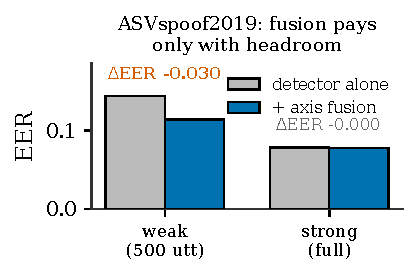
\includegraphics[width=\linewidth]{figs/fig_fusion_asvspoof.pdf}
\caption{ASVspoof2019.}
\label{fig:fuse-asv}
\end{subfigure}\hfill
\begin{subfigure}[t]{0.25\linewidth}
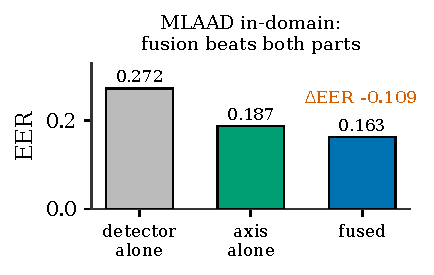
\includegraphics[width=\linewidth]{figs/fig_fusion_mlaad.pdf}
\caption{MLAAD in-domain.}
\label{fig:fuse-mlaad}
\end{subfigure}\hfill
\begin{subfigure}[t]{0.34\linewidth}
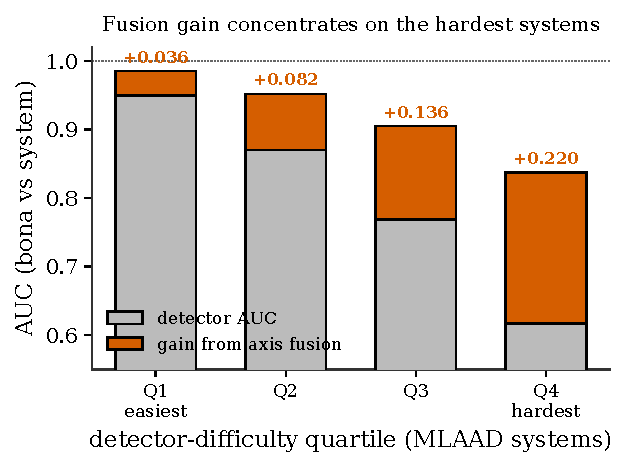
\includegraphics[width=\linewidth]{figs/fig3_quartile_mechanism.pdf}
\caption{Gain vs.\ difficulty.}
\label{fig:quartile}
\end{subfigure}
\caption{\textbf{(a)}~The same recipe cuts a weak ASVspoof2019 detector's EER
($0.144\!\to\!0.114$) but leaves a strong, near-ceiling one unchanged.
\textbf{(b)}~In-domain on MLAAD, fusion ($0.163$) beats detector-alone ($0.272$)
and axis-alone ($0.187$). \textbf{(c)}~Fusion's AUC gain rises from $+0.036$
(easiest MLAAD quartile) to $+0.220$ (hardest).}
\label{fig:fusion}
\vspace{-10pt}
\end{figure}

\textbf{Headroom decides.} A deliberately weak WavLM-GAT trained on 500 utterances
drops from EER $0.144$ to $0.114$ under the unsupervised axis ($\Delta$EER
$=-0.030$, 95\% CI $[-0.046,-0.013]$, $p\approx0$), improving all five
attack-disjoint folds---a $\approx$21\% reduction (Fig.~\ref{fig:fuse-asv}). The
identical procedure on a strong, near-ceiling WavLM-GAT (EER $0.078$) produces no
change beyond noise ($\Delta$EER $=-0.0004$ to $+0.004$, $p\approx0.56$--$0.80$).
In-domain on MLAAD, likewise far from ceiling, the same centroid fusion improves
EER from $0.272$ to $0.163$ (axis alone $0.187$), negative across all folds and
seeds (Fig.~\ref{fig:fuse-mlaad}).

\textbf{Why the axis works.} The gain lands on the hardest systems. By MLAAD
detector-difficulty quartile, fusion's AUC gain grows monotonically from $+0.036$
(easiest) to $+0.220$ (hardest) (Fig.~\ref{fig:quartile})---the law turned into
performance. Hard systems sit close to bona-fide speech with high spread along a
direction the detector under-weights, so re-injecting it recovers exactly them; a
strong detector has already learned the direction and gains nothing---the headroom
condition follows from the mechanism.

\section{Limitations and conclusion}
The law is text-to-speech-specific: on voice conversion all predictors give
$\rho\approx0$, as converted speech inherits its content, and spread, from source
speech. Geometry uses one backbone (WavLM; wav2vec\,2.0 \citep{baevski2020wav2vec}
and HuBERT \citep{hsu2021hubert} untested), and the causal contrasts rest on three
seeds---trustworthy in sign, not in power. Cross-dataset \emph{prospective}
prediction is unconfirmed: a pre-registered, externally timestamped test on
held-out ASVspoof-2021-DF failed honestly ($\rho=+0.33$, $p=0.135$, $n=13$),
reported not omitted. Within these bounds, a low-cost, frozen, training-free
direction genuinely helps understand and partially correct detectors---for weak
detectors within a dataset, not across datasets or for strong ones.

\subsubsection*{Reproducibility statement}
All results use a single-GPU pipeline: a frozen $\sim$95M-parameter encoder
(WavLM-base, 94.7M) and a $\sim$13M head ($\ll 3$B parameters), largest run
$\approx 10^{16}$ FLOPs. Every number regenerates from a committed script over
cached embeddings, released with logs, checkpoints, and the audit.

\bibliography{references}
\bibliographystyle{colm2026_conference}

\end{document}
